%----------------------------------------------------------------------------
%----------------------------------------------------------------------------
The average behavior of the ensemble from Section \ref{model} is modeled using the formalism from Section \ref{density formalism}. Since the stochastic model conserves probability (the collision does not change the magnitude of the expansion coefficients) $\hat{R}^{ext}$ is set to zero. If $\hat{R}^{int}=0$ then a computer fit converges on the obvious solution quickly: namely the $\gamma_{ij}$'s in Equation \ref{dephase3} are all equal to the probability of a collision per unit time ($0.5/\pi$ in Figures \ref{coll_1}, \ref{coll_2}, and \ref{average}).

A more interesting check would be to see if we can distinguish between the two probability conserving terms in Equation \ref{R} ($\hat{R}^{int}$ and $\hat{R}^{phase}$) by only using the diagonals of the density matrix. The diagonal terms of the density matrix represent the probability of finding the system in a particular state -- thus easily observable in an experiment. The number of free parameters in the fit is reduced (to keep the program run time less than a day) by assuming that probability only ``leaks'' down so that only $\Gamma^{2}_{0}$, $\Gamma^{1}_{0}$, and $\Gamma^{2}_{1}$ are non-zero among the elements of $\hat{R}^{int}$. This is a reasonable assumption if spontaneous emission is the dominant relaxation process (other than collisions).

Now the density matrix reduces to six coupled differential equations:
%----------------------------------------------------------------------------
\begin{subequations}
\begin{eqnarray}
\dot{\rho}_{00}&=&
+\Gamma^{1}_{0}\rho_{11} + \Gamma^{2}_{0}\rho_{22}
- \alpha (\rho_{01} + \rho_{10})\\
\dot{\rho}_{11}&=&
-\Gamma^{1}_{0}\rho_{11} + \Gamma^{2}_{1}\rho_{22}
+ \alpha (\rho_{01} + \rho_{10}) - \beta (\rho_{21} + \rho_{12})\\
\dot{\rho}_{22}&=&
-\Gamma^{2}_{0}\rho_{22} - \Gamma^{2}_{1}\rho_{22}
+ \beta (\rho_{12} + \rho_{21})\\
\dot{\rho}_{01}&=&
-\gamma_{01}\rho_{01}
+ \alpha (\rho_{00} - \rho_{11}) - \beta\rho_{02}\\
\dot{\rho}_{02}&=&
-\gamma_{02}\rho_{02}
+ \beta\rho_{01} - \alpha\rho_{12}\\
\dot{\rho}_{12}&=&
-\gamma_{12}\rho_{12}
+ \alpha\rho_{02} + \beta (\rho_{11} - \rho_{22})
\end{eqnarray}
\label{fit dynamics}
\end{subequations}
%----------------------------------------------------------------------------
Clearly, the $\Gamma$'s should all be zero since the original model from Section \ref{model} did not include any population transfer; however, for this ``test'' we will keep them and see if a computer fit can show the $\Gamma$'s to be zero using only the occupation probabilities. In an actual experiment, we may only have access to the occupation probabilities, so this situation is somewhat realistic.

To compare this model to the average ensemble behavior from Section \ref{model} a cost function, based off of the diagonals of the density matrix, is defined:
%----------------------------------------------------------------------------
\begin{equation}
\Theta(\Gamma^{1}_{0},\Gamma^{2}_{0},\Gamma^{2}_{1},\gamma_{01},\gamma_{02},\gamma_{12})\equiv
\sum_{n,i}
\left(
P_{i}(t_n) - P^{\prime}_{i}(t_n)
\right)^2
\label{the cost function}
\end{equation}
%----------------------------------------------------------------------------
where the sum is taken over the number of time points $n=0,1,\ldots,999$ and the number of states $i=0,1,2$. This cost function will be large (small) if there is a large (small) difference between the dynamics from Section \ref{model} and the density matrix dynamics; thus, we would like to minimize this cost function as a function of the gamma coefficients. The terms in the sum are
%----------------------------------------------------------------------------
\begin{equation}
P_i
\equiv
c_i \cdot c^{*}_i
\end{equation}
%----------------------------------------------------------------------------
for the ``state vector'' approach ($c_i$ is the expansion coefficient in the average ensemble behavior from Section \ref{model}) and
%----------------------------------------------------------------------------
\begin{equation}
P^{\prime}_{i}\equiv
\rho_{ii}
\end{equation}
%----------------------------------------------------------------------------
 for the ``density matrix'' approach from Section \ref{density formalism} where  and $\rho_{ii}$ is from Equation \ref{fit dynamics} (and thus a function of $\Gamma^{1}_{0},\Gamma^{2}_{0},\Gamma^{2}_{1},\gamma_{01},\gamma_{02},$ and $\gamma_{12}$).
%----------------------------------------------------------------------------

Two simulations were run: one with the collision probability set to 0.5/$\pi$ and one with the collision probability set to 0.3/$\pi$. Figures \ref{coll_1} and \ref{coll_2} show individual runs that are then averaged with many other runs to produce an approximation to ensemble behavior as shown in Figure \ref{average}.
%----------------------------------------------------------------------------
%----------------------------------------------------------------------------
%bb defines the bounding box for the pdf
%viewport defines the area of the pdf used
%in sidewaysfigure the last entry in bb moves the caption toward/away the pic
%in sidewaysfigure the second entry in bb moves the pic toward/away the caption
%----------------------------------------------------------------------------
\begin{figure}
\scalebox{0.8}[0.8]{
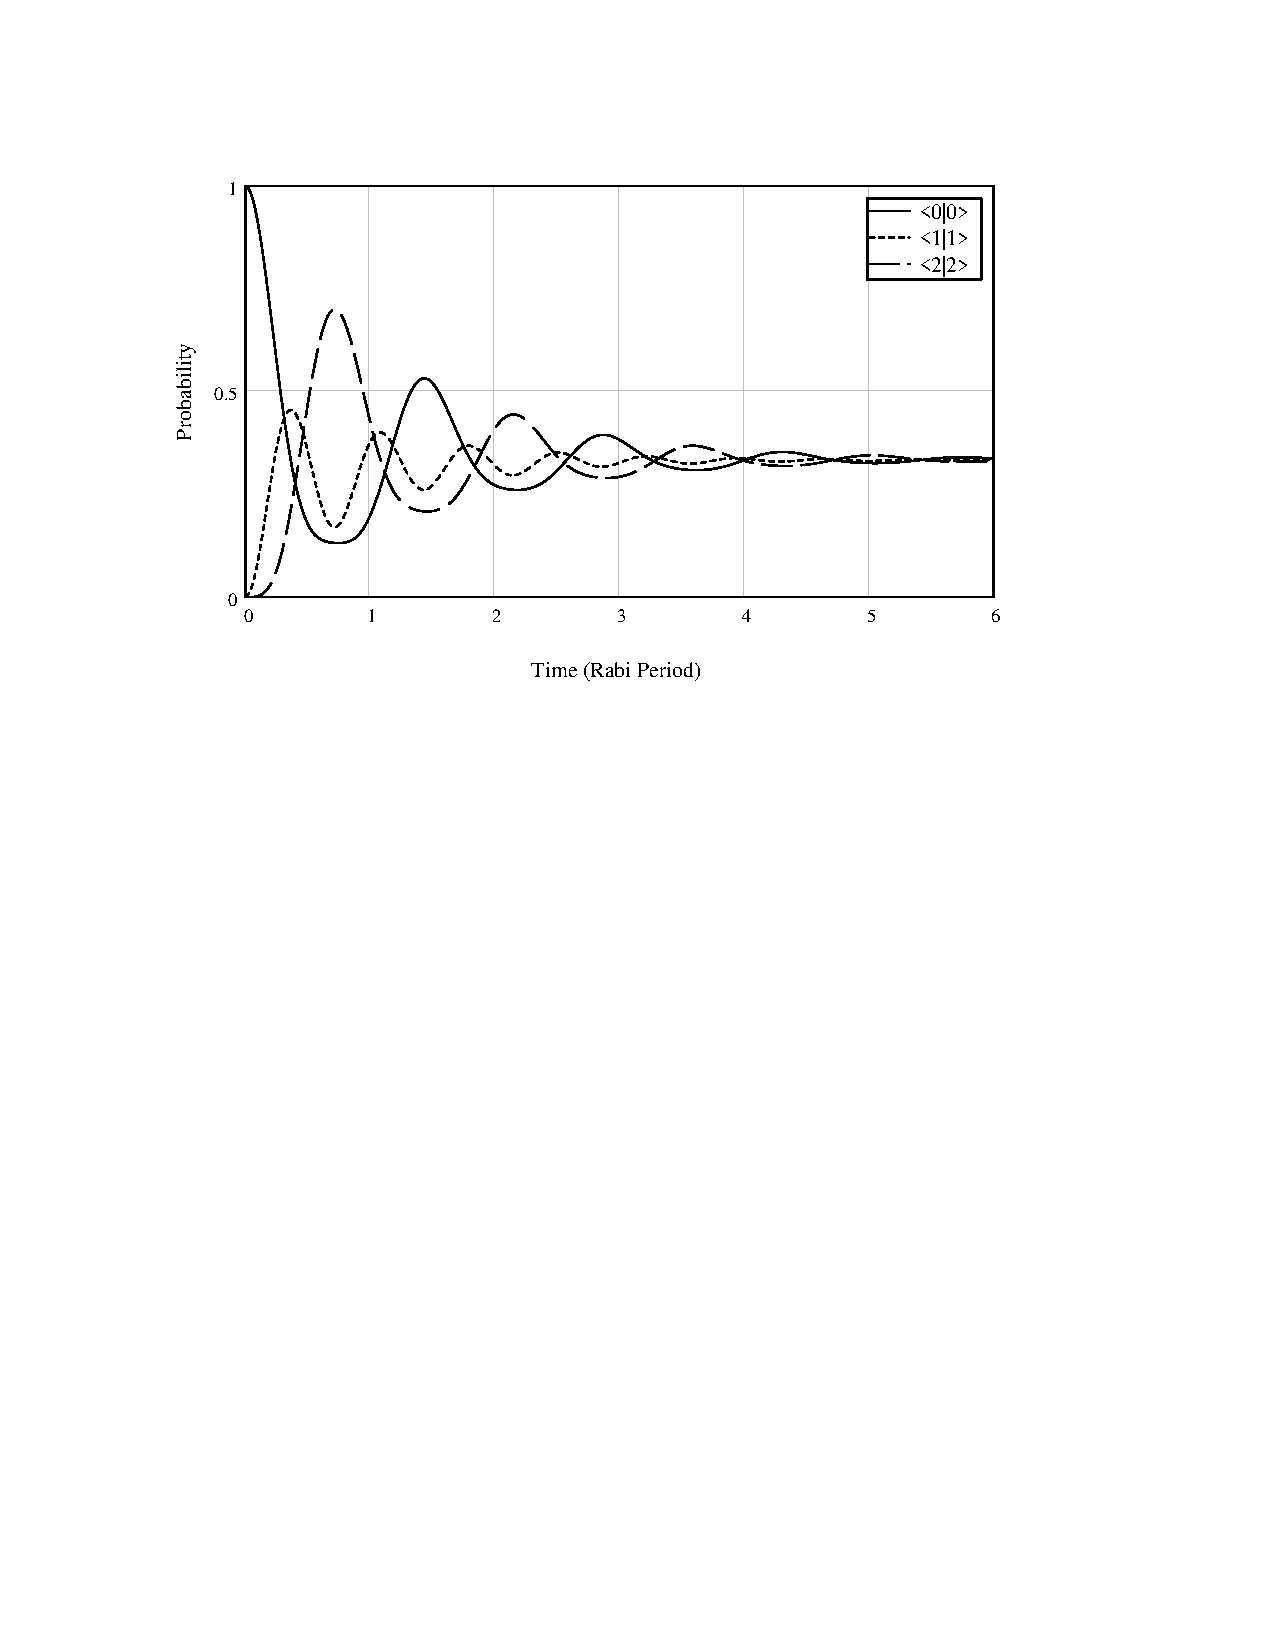
\includegraphics[bb=30 455 489 685]
{average/average.pdf}
}
\caption[Average dynamics of one million stochastic runs]{One million runs like those shown in Figure \ref{coll_1} and \ref{coll_2} are averaged to produce the plot shown above. The six parameter fit is so close that the difference is not perceptible at this scale.}
\label{average}
\end{figure}
%----------------------------------------------------------------------------

%----------------------------------------------------------------------------
The ``Simplex'' parameter optimization method is used \cite{Press:1992a} to minimize the cost function, Equation \ref{the cost function}, as a function of $\Gamma^{1}_{0},\Gamma^{2}_{0},\Gamma^{2}_{1},\gamma_{01},\gamma_{02},$ and $\gamma_{12}$). For a simulation where the collision probability set to 0.5/$\pi$ we get
%----------------------------------------------------------------------------
\begin{subequations}
\begin{eqnarray}
\Gamma^{1}_{0}&=&
0.490795/\pi\\
\Gamma^{2}_{0}&=&
0.255223/\pi\\
\Gamma^{2}_{1}&=&
0.488124/\pi\\
\gamma_{10}&=&
0.00183362/\pi\\
\gamma_{02}&=&
0.315977/\pi\\
\gamma_{12}&=&
3.72062\cross10^{-5}/\pi,
\end{eqnarray}
\end{subequations}
%----------------------------------------------------------------------------
with $\Theta=0.00648676$ (1000 points) and for a simulation where the collision probability set to 0.3/$\pi$ we get
%----------------------------------------------------------------------------
\begin{subequations}
\begin{eqnarray}
\Gamma^{1}_{0}&=&
0.290149/\pi\\
\Gamma^{2}_{0}&=&
0.151391/\pi\\
\Gamma^{2}_{1}&=&
0.288282/\pi\\
\gamma_{10}&=&
0.00650929/\pi\\
\gamma_{02}&=&
0.173519/\pi\\
\gamma_{12}&=&
0.00260537/\pi.
\end{eqnarray}
\end{subequations}
%----------------------------------------------------------------------------
with $\Theta=0.00360311$ (1000 points).

The fact that the simulations fit the data very well is not that encouraging since the fit had six parameters. The results are characteristically nebulous with $\Gamma^{1}_{0}$ and $\Gamma^{2}_{1}$ apparently absorbing the effect while $\Gamma^{2}_{0}$ and $\gamma_{02}$ seem to split responsibility in both simulations. It appears that internal probability damping ($\hat{R}^{int}$) may be indistinguishable from phase damping ($\hat{R}^{phase}$) when only observing state occupation probability in the collisional model. This could be further checked by running two different fits which depend only on $\hat{R}^{int}$ or $\hat{R}^{phase}$ and comparing the results and/or running a simulation with the pulse on for the first half and off for the second half. Once a method of assigning realistic magnitudes to the elements of these relaxation matrices is found, this formalism can be used to numerically explore the effects of relaxation on coherent control schemes.
%----------------------------------------------------------------------------
%----------------------------------------------------------------------------
%----------------------------------------------------------------------------
